\section{Clustering results on the proposed data set}\label{Clustering}

\subsection{About Clustering}

Clustering is a process of grouping items together based on their distance \parencite{likas2003global}. Lets take the image from bellow as an example. We have 3 classes (red, green and blue). Model calculates the distances between items (nodes) and classifies them based on how close are they between each other.

\begin{figure}[H]
    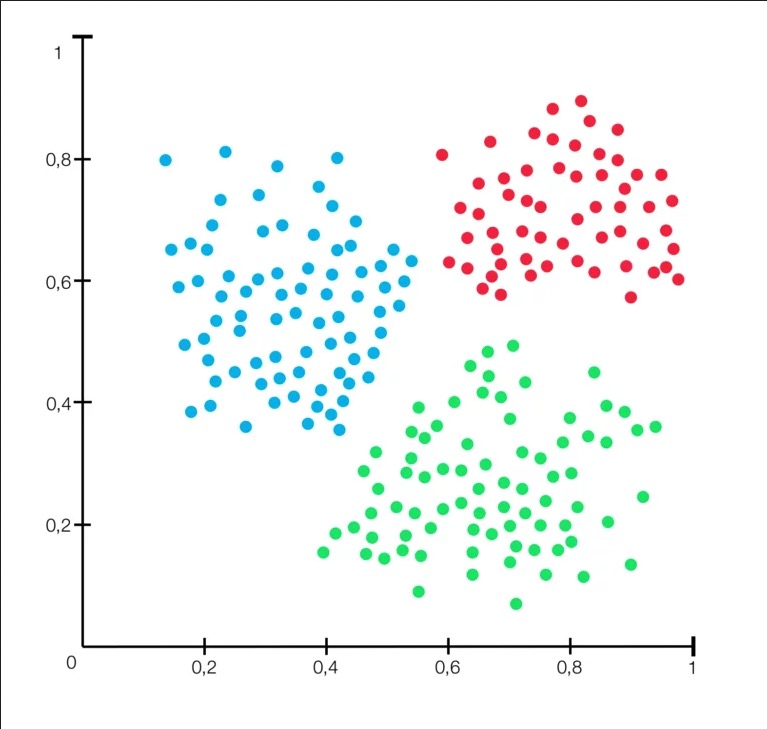
\includegraphics[scale=0.30]{img/Clustering/Clustering.jpg}
    \centering
    \caption{Clustering \parencite{web:Rocketloop}}
    \label{fig:clustering}
\end{figure}

Further explanation can be seen at \ref{A3}.

Code bellow showcases how we split the data. It is similar to classification.
\begin{listing}[H]
\caption{Split data function}
\begin{minted}{python}
def train_test_split(dataframe, test_ratio=0.2):
    dataframe = dataframe.withColumn('strength', col('strength').cast('double'))

    train_df, test_df = dataframe.randomSplit
                        ([1 - test_ratio, test_ratio], seed=42)

    return train_df, test_df
\end{minted}
\end{listing}

\newpage
\subsection{K-means}

\subsubsection{About}

K-means is a clustering algorithm \parencite{hartigan1979algorithm}. It is one of the more popular algorithms used for clustering. How it usually works is by us providing k (number of clusters) to the algorithm. Our model will then calculate the distance (there are different calculations: Euclidean, Manhattan, etc...) between nodes. Afterwards we can see the ideal number and chose it as our number of clusters.
\newpage
\subsubsection{Implementation}

Implementation is similar to decision tree. We are expecting training data in the function, select platform type as what to predict and vectorise he data. SVM can be optimised as well, grid was used (same as with decision trees) and cross validation was applied as well. At the end, SVM model is returned.
\begin{listing}[H]
\caption{SVM model function}
\begin{minted}{python}
def build_svm_model(x_train, y_train):
    train_data = spark.createDataFrame
                 (pd.concat([x_train, y_train], axis=1))

    platform_indexer = StringIndexer(inputCol="platformType", 
                                     outputCol="indexedLabel")
    train_data = platform_indexer.fit(train_data).transform(train_data)

    assembler = VectorAssembler(inputCols=["indexedLabel"], 
                                outputCol="features")
    train_data = assembler.transform(train_data)

    svm = LinearSVC(featuresCol="features", labelCol="indexedLabel")

    paramGrid = ParamGridBuilder() \
        .addGrid(svm.maxIter, [10, 100]) \
        .addGrid(svm.regParam, [0.1, 0.01]) \
        .build()

    ovr = OneVsRest(classifier=svm)

    evaluator = MulticlassClassificationEvaluator(labelCol="indexedLabel", 
                predictionCol="prediction", metricName="accuracy")
    crossval = CrossValidator(estimator=ovr, estimatorParamMaps=paramGrid, 
                              evaluator=evaluator, numFolds=5)

    cvModel = crossval.fit(train_data)

    return cvModel.bestModel
\end{minted}
\end{listing}




























% \begin{listing}[H]
% \caption{Evaluate SVM model}
% \begin{minted}{python}
% evaluate_model(svm_model, x_test, y_test, file_Path = file_paths_dict["classification"] + "SVM")
% \end{minted}
% \end{listing}

\newpage
\subsubsection{Results}

At the end, we need to evaluate the model in order to get the results. We pass in our model, test data and location where we want results to be saved. The function (that is split into parts 1-4) then evaluates the model and results are available to us.
\begin{listing}[H]
\caption{Evaluate model model function -part 1}
\begin{minted}{python}
def evaluate_model(model, x_test, y_test, file_Path):
    test_data = spark.createDataFrame
                (pd.concat([x_test, y_test], axis=1))

    platform_indexer = StringIndexer(inputCol="platformType", 
                                    outputCol="platformIndex")
    test_data = platform_indexer.fit(test_data).transform(test_data)

    assembler = VectorAssembler(inputCols=["platformIndex"], 
                                outputCol="features")
    test_data = assembler.transform(test_data)

    predictions = model.transform(test_data)

    evaluator = MulticlassClassificationEvaluator(labelCol="label", 
                                        predictionCol="prediction")

    class_labels = test_data.select("label").distinct()
                    .rdd.flatMap(lambda x: x).collect()
    metrics = {}

\end{minted}
\end{listing}

\begin{listing}[H]
\caption{Evaluate model model function -part 2}
\begin{minted}{python}
    for label in class_labels:
        evaluator.setMetricName("accuracy")
        evaluator.setMetricLabel(label)
        accuracy = evaluator.evaluate(predictions)

        evaluator.setMetricName("weightedPrecision")
        evaluator.setMetricLabel(label)
        precision = evaluator.evaluate(predictions)

        evaluator.setMetricName("weightedRecall")
        evaluator.setMetricLabel(label)
        recall = evaluator.evaluate(predictions)

        evaluator.setMetricName("weightedFMeasure")
        evaluator.setMetricLabel(label)
        f1_score = evaluator.evaluate(predictions)

\end{minted}
\end{listing}

\begin{listing}[H]
\caption{Evaluate model model function -part 3}
\begin{minted}{python}
        metrics[label] = {"accuracy": accuracy, "precision": precision, 
                          "recall": recall, "f1-score": f1_score}

    predictionAndLabels = predictions.select("prediction", "label").rdd
    multiclass_metrics = MulticlassMetrics(predictionAndLabels)
    confusion_matrix = multiclass_metrics.confusionMatrix().toArray()

    label_counts = predictionAndLabels.map(lambda x: (x[1], 1))
                   .reduceByKey(lambda x, y: x + y).collectAsMap()
    support = {label: label_counts.get(label, 0) for label in class_labels}

    metrics_table = pd.DataFrame.from_dict(metrics, orient="index")
    print("Metrics per Class:")
    print(metrics_table)

    support_table = pd.DataFrame.from_dict
                    (support, orient="index", columns=["Support"])
    print("Support:")
    print(support_table)

    fig, ax = plt.subplots()
    im = ax.imshow(confusion_matrix, cmap="Blues")

    tick_labels = np.arange(len(class_labels))
    ax.set_xticks(tick_labels)
    ax.set_yticks(tick_labels)
    ax.set_xticklabels(class_labels, rotation=45)
    ax.set_yticklabels(class_labels)
    plt.xlabel("Predicted")
    plt.ylabel("Actual")
\end{minted}
\end{listing}

\begin{listing}[H]
\caption{Evaluate model model function -part 4}
\begin{minted}{python}
    cbar = ax.figure.colorbar(im, ax=ax)
    cbar.ax.set_ylabel("Count", rotation=-90, va="bottom")

    for i in range(len(class_labels)):
        for j in range(len(class_labels)):
            text = ax.text(j, i, int(confusion_matrix[i, j]), 
                           ha="center", va="center", color="w")

    plt.title("Confusion Matrix")
    
    metrics_table.to_csv(file_Path + "/metrics.csv")
    plt.savefig(file_Path + "/confusion_matrix.png")

    plt.close()
\end{minted}
\end{listing}

\begin{figure}[H]
    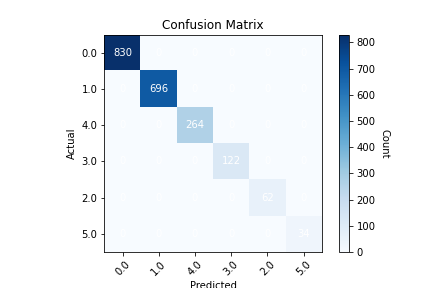
\includegraphics[scale=0.85]{img/Model/Classification/Dtree/confusion_matrix.png}
    \centering
    \caption{Decision tree confusion matrix}
    \label{fig:dtree_confusion_matrix}
\end{figure}
\newpage
\newpage
\subsection{GMM}

\subsubsection{About}

K-means is a clustering algorithm \parencite{hartigan1979algorithm}. It is one of the more popular algorithms used for clustering. How it usually works is by us providing k (number of clusters) to the algorithm. Our model will then calculate the distance (there are different calculations: Euclidean, Manhattan, etc...) between nodes. Afterwards we can see the ideal number and chose it as our number of clusters.
\newpage
\subsubsection{Implementation}

Implementation is similar to decision tree. We are expecting training data in the function, select platform type as what to predict and vectorise he data. SVM can be optimised as well, grid was used (same as with decision trees) and cross validation was applied as well. At the end, SVM model is returned.
\begin{listing}[H]
\caption{SVM model function}
\begin{minted}{python}
def build_svm_model(x_train, y_train):
    train_data = spark.createDataFrame
                 (pd.concat([x_train, y_train], axis=1))

    platform_indexer = StringIndexer(inputCol="platformType", 
                                     outputCol="indexedLabel")
    train_data = platform_indexer.fit(train_data).transform(train_data)

    assembler = VectorAssembler(inputCols=["indexedLabel"], 
                                outputCol="features")
    train_data = assembler.transform(train_data)

    svm = LinearSVC(featuresCol="features", labelCol="indexedLabel")

    paramGrid = ParamGridBuilder() \
        .addGrid(svm.maxIter, [10, 100]) \
        .addGrid(svm.regParam, [0.1, 0.01]) \
        .build()

    ovr = OneVsRest(classifier=svm)

    evaluator = MulticlassClassificationEvaluator(labelCol="indexedLabel", 
                predictionCol="prediction", metricName="accuracy")
    crossval = CrossValidator(estimator=ovr, estimatorParamMaps=paramGrid, 
                              evaluator=evaluator, numFolds=5)

    cvModel = crossval.fit(train_data)

    return cvModel.bestModel
\end{minted}
\end{listing}




























% \begin{listing}[H]
% \caption{Evaluate SVM model}
% \begin{minted}{python}
% evaluate_model(svm_model, x_test, y_test, file_Path = file_paths_dict["classification"] + "SVM")
% \end{minted}
% \end{listing}

\newpage
\subsubsection{Results}

At the end, we need to evaluate the model in order to get the results. We pass in our model, test data and location where we want results to be saved. The function (that is split into parts 1-4) then evaluates the model and results are available to us.
\begin{listing}[H]
\caption{Evaluate model model function -part 1}
\begin{minted}{python}
def evaluate_model(model, x_test, y_test, file_Path):
    test_data = spark.createDataFrame
                (pd.concat([x_test, y_test], axis=1))

    platform_indexer = StringIndexer(inputCol="platformType", 
                                    outputCol="platformIndex")
    test_data = platform_indexer.fit(test_data).transform(test_data)

    assembler = VectorAssembler(inputCols=["platformIndex"], 
                                outputCol="features")
    test_data = assembler.transform(test_data)

    predictions = model.transform(test_data)

    evaluator = MulticlassClassificationEvaluator(labelCol="label", 
                                        predictionCol="prediction")

    class_labels = test_data.select("label").distinct()
                    .rdd.flatMap(lambda x: x).collect()
    metrics = {}

\end{minted}
\end{listing}

\begin{listing}[H]
\caption{Evaluate model model function -part 2}
\begin{minted}{python}
    for label in class_labels:
        evaluator.setMetricName("accuracy")
        evaluator.setMetricLabel(label)
        accuracy = evaluator.evaluate(predictions)

        evaluator.setMetricName("weightedPrecision")
        evaluator.setMetricLabel(label)
        precision = evaluator.evaluate(predictions)

        evaluator.setMetricName("weightedRecall")
        evaluator.setMetricLabel(label)
        recall = evaluator.evaluate(predictions)

        evaluator.setMetricName("weightedFMeasure")
        evaluator.setMetricLabel(label)
        f1_score = evaluator.evaluate(predictions)

\end{minted}
\end{listing}

\begin{listing}[H]
\caption{Evaluate model model function -part 3}
\begin{minted}{python}
        metrics[label] = {"accuracy": accuracy, "precision": precision, 
                          "recall": recall, "f1-score": f1_score}

    predictionAndLabels = predictions.select("prediction", "label").rdd
    multiclass_metrics = MulticlassMetrics(predictionAndLabels)
    confusion_matrix = multiclass_metrics.confusionMatrix().toArray()

    label_counts = predictionAndLabels.map(lambda x: (x[1], 1))
                   .reduceByKey(lambda x, y: x + y).collectAsMap()
    support = {label: label_counts.get(label, 0) for label in class_labels}

    metrics_table = pd.DataFrame.from_dict(metrics, orient="index")
    print("Metrics per Class:")
    print(metrics_table)

    support_table = pd.DataFrame.from_dict
                    (support, orient="index", columns=["Support"])
    print("Support:")
    print(support_table)

    fig, ax = plt.subplots()
    im = ax.imshow(confusion_matrix, cmap="Blues")

    tick_labels = np.arange(len(class_labels))
    ax.set_xticks(tick_labels)
    ax.set_yticks(tick_labels)
    ax.set_xticklabels(class_labels, rotation=45)
    ax.set_yticklabels(class_labels)
    plt.xlabel("Predicted")
    plt.ylabel("Actual")
\end{minted}
\end{listing}

\begin{listing}[H]
\caption{Evaluate model model function -part 4}
\begin{minted}{python}
    cbar = ax.figure.colorbar(im, ax=ax)
    cbar.ax.set_ylabel("Count", rotation=-90, va="bottom")

    for i in range(len(class_labels)):
        for j in range(len(class_labels)):
            text = ax.text(j, i, int(confusion_matrix[i, j]), 
                           ha="center", va="center", color="w")

    plt.title("Confusion Matrix")
    
    metrics_table.to_csv(file_Path + "/metrics.csv")
    plt.savefig(file_Path + "/confusion_matrix.png")

    plt.close()
\end{minted}
\end{listing}

\begin{figure}[H]
    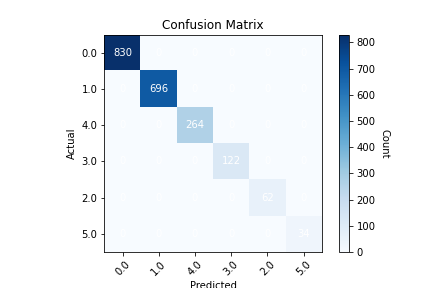
\includegraphics[scale=0.85]{img/Model/Classification/Dtree/confusion_matrix.png}
    \centering
    \caption{Decision tree confusion matrix}
    \label{fig:dtree_confusion_matrix}
\end{figure}
\newpage


\subsection{Execute clustering code}
Code bellow is the main part that calls the functions in order to generate the models and evaluates the models.

As seen in results section, or models performed quite well. K-means seems to be the most efficient with about 30-34 clusters while GNN seems to be happy with 100 distributions.
\begin{listing}[H]
\caption{Execute the classification functions}
\begin{minted}{python}
train_df, test_df = train_test_split(mega_dataframe)
train_df, test_df = train_test_split(mega_dataframe)

evaluate_kmeans_model(train_df, test_df, 50, 
file_Path = file_paths_dict["clustering"] + "kmenas")

evaluate_gmm_model(train_df, test_df, 200, 
file_Path = file_paths_dict["clustering"] + "gmm")

\end{minted}
\end{listing}
